\subsection{Methodology}

For this project team decided to use an adoption of the SCRUM methodology, an agile methodology. Other option was to use waterfall model. After the preliminary study, it is considered inappropriate, as it requires very strict definition of user requirements before beginning of development process. It is expected that user requirements may change significantly during the development of the application, and in the beginning project and domain are still very loosely defined. In addition, the customer and the advisor from IDI recommended use of an agile methodology. More about choice of development process in section 'Preliminary study'.

Planned work will consist of daily stand-up meetings, where all group members will be present and discuss about issues completed during previous day and plans for the following day. Beside this, main internal group meeting will be held on Mondays, and meetings with advisor and customer will mostly be scheduled for Tuesday. Each sprint will be planned on internal meetings and at the end of sprint results will be presented to both customer and advisor. Sprint plan will also be agile, taking into consideration the ever changing requirements. Team will have product owner and scrum master, but will not strictly employ standards such as SCRUM board. 

\subsection{Project phases}

Our project will loosely follow the plan in Figure~\ref{gantt:project}.

\begin{figure}[h]
\centering
  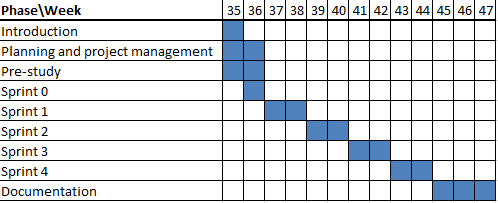
\includegraphics[width=1.0\textwidth]{project_management/project_effort_estimation}
  \caption[Gantt chart of project phases]{Gantt chart showing project phases, and when they are planned done.}
  \label{gantt:project}
\end{figure}
First week for this project is planed like introductory week, where team members will get introduced to each other and get familiar with project and following assignments.\newline
After that, first official phase of the project lasts for 2 weeks, and refers to planing and project management. During this period all administrative tasks should be finished, allowing smooth start of actual developing process. At the same time, preliminary study will be one of the occupations for all team members. This should give clear picture of technologies, development processes and project work flow for upcoming months.\newline
Beginning of actual development is scheduled for week 36, overlapping with previous phase. Development process will consist of this so called zero sprint, lasting 1 week, and four 2-week sprints. At the end of sprint 4, week 44, team should finish application development and provide release version to customer.\newline
Last 3 weeks are reserved for finishing documentation, which was written throughout whole previous phases. During this period, remaining sections should be finished, whole document thoroughly revised and prepared for final delivery.\newline

\subsubsection{Planning and research}

This first phase of the project consists of an introduction to the course,
planning of the project, introduction to the problem domain, getting to know
the group, requirement gathering and such. In this phase the most important
decisions about system architecture, choice of COTS and framework, project
methodology and role distribution, will be taken. Figure~\ref{gantt:pre_imp}
shows how the work will be distributed in this time period.

\begin{figure}[h]
\centering
  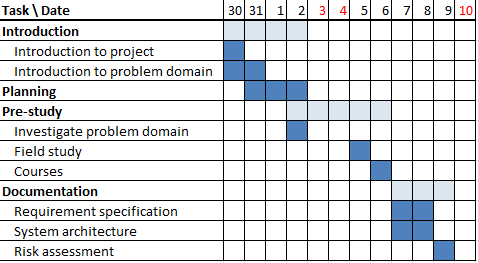
\includegraphics[width=1.0\textwidth]{project_management/pre_implementation_gantt}
  \caption[Gantt chart of planning and research phase]{Gantt diagram picturing how work should be distributed in the time available during the planning and research phase.}
  \label{gantt:pre_imp}
\end{figure}

\subsubsection{Sprints}

Each sprint will consist of four phases. Effort estimation is
detailed in Table \ref{Sprint effort estimation}.

\begin{table}[htbp]
\begin{center}
  \begin{tabular}{|r|r|r|}
    \hline
    \bf{Task} & \bf{Hours per person} & \bf{Hours total} \\
    \hline
    Planning & 8 & 56 \\
    Implementation & 8 & 56 \\
    Testing & 8 & 56 \\
    Documentation & 16 & 112 \\
    Administrative & 8 & 56 \\
    \hline \hline
    \bf{Sum} & 50 & 350 \\
    \hline
  \end{tabular}
  \caption{Task effort estimation for each sprint}
  \label{Sprint effort estimation}
\end{center}
\end{table}

\textbf{Planning} The planning phase of each sprint represents the time
required for work distribution, planning of how each task should be handled,
and how testing should be done for this section.

\textbf{Implementation} The implementation phase represents time spent on coding.
This will also include code refactoring and other maintenance tasks
related to the code.

\textbf{Testing} The testing phase represents time spent testing the system.
This includes integration testing, unit testing, functional testing etc.
The testing and implementation phases will work concurrently due to the
test-driven development methodology.

\textbf{Documentation} The documentation phase represents time spent
documenting work effort (implementation, research, etc.) and administrative
tasks like meetings.

\subsubsection{Documentation}
The last part of the project will consist of evaluating our work, and finish the documentation of the project. In addition, this part will include a final presentation November 24th for the external examiner, advisor and customer. This period will span the last three weeks of the project.  
